\documentclass{article}
\usepackage[utf8]{inputenc} %кодировка
\usepackage[T2A]{fontenc}
\usepackage[english,russian]{babel} %русификатор 
\usepackage{mathtools} %библиотека матеши
\usepackage[left=1cm,right=1cm,top=2cm,bottom=2cm,bindingoffset=0cm]{geometry} %изменение отступов на листе
\usepackage{amsmath}
\usepackage{graphicx} %библиотека для графики и картинок
\graphicspath{}
\DeclareGraphicsExtensions{.pdf,.png,.jpg}
\usepackage{subcaption}
\usepackage{pgfplots}

\begin{document}

\section{Инфологические модели и даталогические}
\textbf{Нужно не менее 6-ти сущностей и связь М:М}

1) Археологические раскопки

археологи(имя, дата рождния, локация, место работы)

должности(название, зарплата)

локации(название, город)

страны(название, дата основания)

города(название, страна, численность населения)

компании(название, престиж)

м:м будет между археологами и должности\\

2) Система контроля версий ПО 

системы контроля(название, актуальность)

проект(название, дата создания, система контроля)

разработчик(имя, дата рождения, должность)

должности(название, зарплата)

файл(название, расширение, дата создания, местоположение)

ветка разработки(название, проект, создатель)

м:м будет между разработчиками и проектами\\

3) Системы распределённого доступа

Пользователь(имя, пароль, роль, индификатор)

Роли(название, дата создания, группа доступа)

Ресурсы(название, тип, сервер)

Сервера(название, группа доступа, индификатор)

Индификаторы(название, страна, тип)

Страны(название, население)

м:м будет между Пользователем и Ресурсами\\

\textbf{Даталогические модели}

1) Археологические раскопки

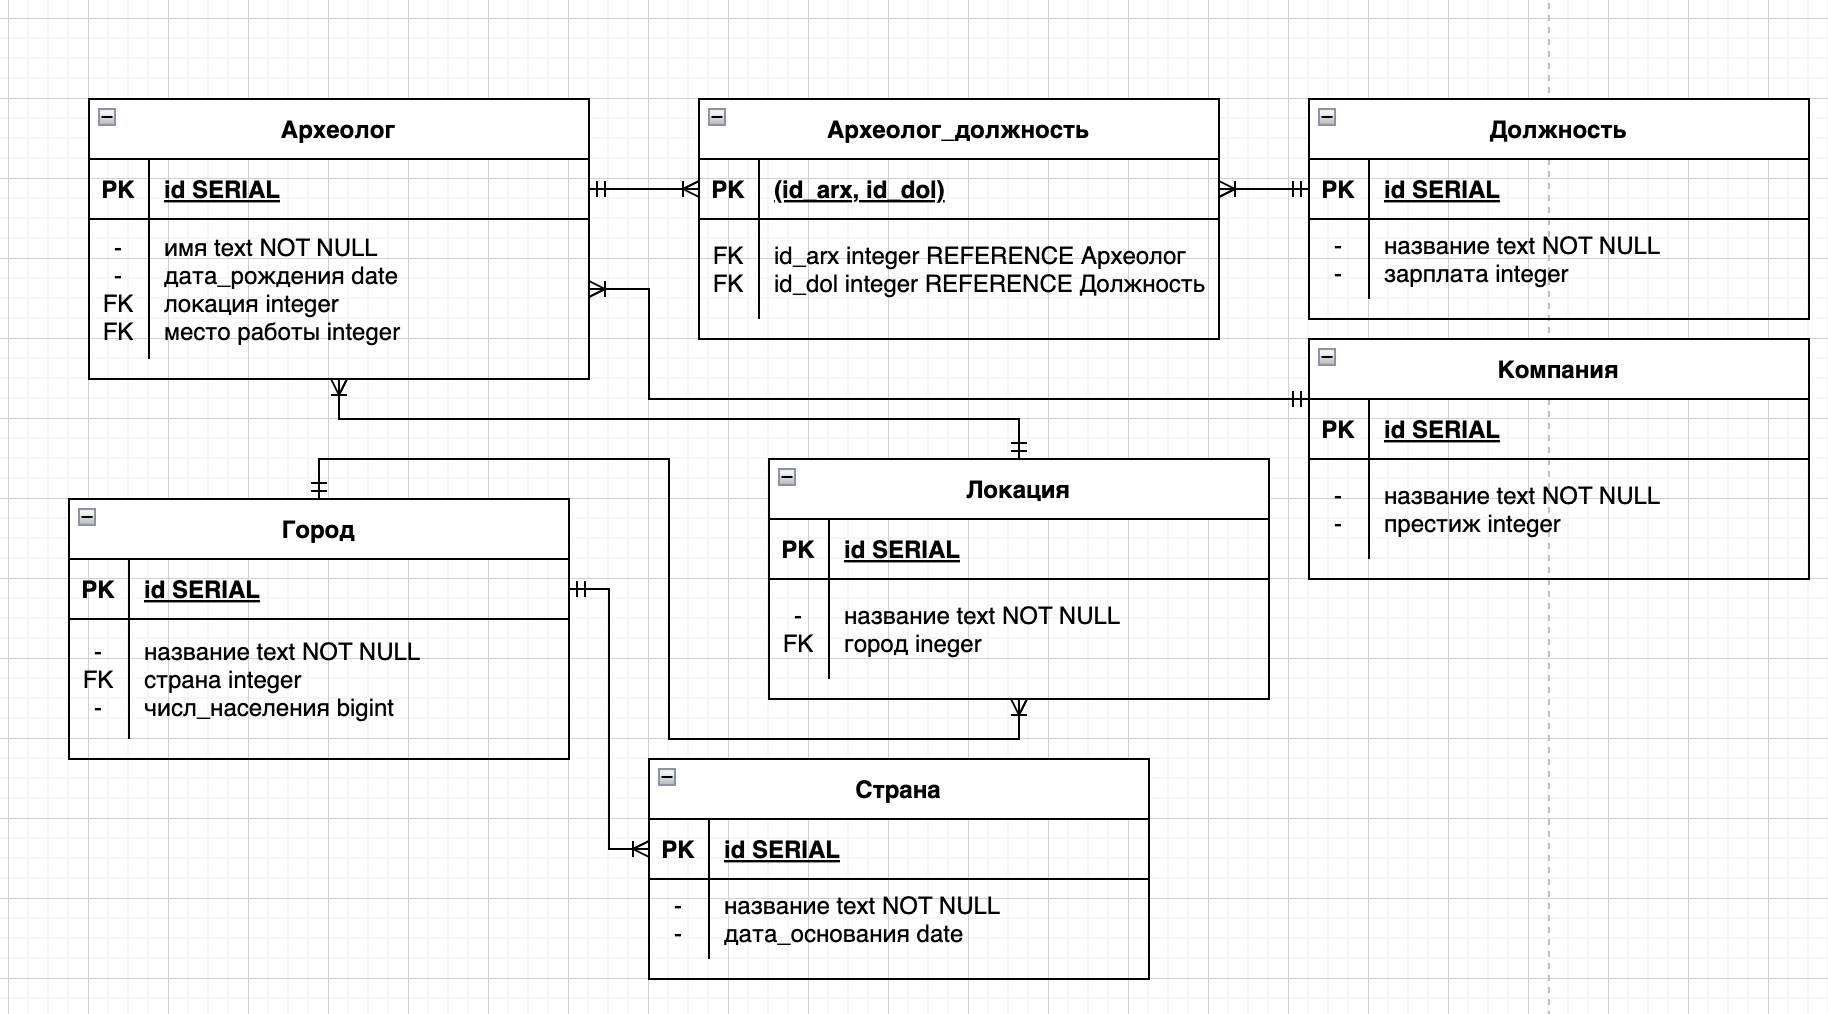
\includegraphics[width=.9\textwidth]{123}
\section{SQL - Запрос}

SELECT Должность.название

FROM Археолог

INNER JOIN Археолог\_должность ON Археолог.id = Археолог\_должность.id

INNER JOIN Должность ON Археолог\_должность.id = Должность.id

WHERE (Должность.зарплата > 10000 AND Археолог.имя = 'Иван');
\\
\\
\textbf{План выполнения}

CREATE INDEX index\_arx ON Археолог (имя) USING HASH;

Используем хеш индекс, так как у нас имеется прямое сравнение.
\\


CREATE INDEX index\_dolj ON Должность USING btree(зарплата);

Используем дерево, чтобы облегчить нахождение первого элемента, который будет > 10000, а далее произойдёт выборка бОльших значений.

\begin{center}
    \begin{tikzpicture}[level distance=1.2cm,
        level 1/.style={sibling distance=2cm},
        level 2/.style={sibling distance=8cm}]
          \node {result}
          child {node {$\pi$ Должность.название}
            child {node {$\bowtie$ Археолог\_должность.id = Должность.id}
            child {node {$\bowtie$ Археолог.id = Археолог\_должность.id}
            child {node {$\sigma $ Археолог.имя = 'Иван'} child {node {Археолог }}}
            child {node {Археолог\_должность}}}
            child {node {$\sigma $ Должность.зарплата > 10000} child {node {Должность }}}
            }};
    \end{tikzpicture}
\end{center}


Этот план выполнения оптимален так как мы достигли цели. На момент соединения строк перебор будет минимальным за счёт отдельных процессов выборки, получилось разделение процессов.

\end{document}
